\documentclass{article}
\usepackage[a4paper, total={7.5in, 10.5in}]{geometry}
\usepackage{graphicx}
\usepackage{wrapfig}
\usepackage{xcolor}
\usepackage{array}
\renewcommand{\baselinestretch}{0.95}
\setlength{\arrayrulewidth}{0.3mm}
\setlength{\tabcolsep}{5pt}
\renewcommand{\arraystretch}{1.7}
\begin{document}
	\begin{wrapfigure}{r}{2cm}
		
	\begin{center}
	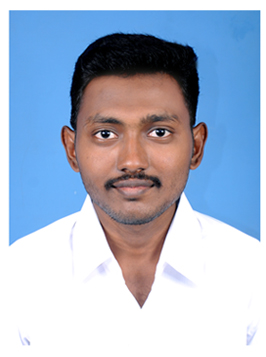
\includegraphics[width=60pt]{Infantraj}
	\end{center}
\end{wrapfigure}
\huge \textbf{\\INFANT RAJ F}  \\
\Large 374/1, AssisiNagar, Sanyasigundu Extn.,\\
Kitchipalayam(P.O), Salem - 636015, TamilNadu, India.\\
Email ID: infantfdr@gmail.com Phone No.:+91 8438383635\\
\hrule 

\Large \textbf{\\Career Objective}\\
\hspace*{20pt} To work in a challenging environment where I can contribute my talents and skills for the optimum growth and development of the organization.

\Large \textbf{\\Education}
\begin{table}[h!]
	\begin{center}
		\begin{tabular}{| m{2cm} | m{5.6cm} | m{3cm} | m{3cm} | m{3.6cm} |}
			\hline
			\Large\centering\textbf{Course} & \Large\centering\textbf{Institution} & \Large\centering \textbf{Board/\\University} & \Large\centering\textbf{Year\hspace{50pt}of Passing} & \Large\hspace{6pt}\textbf{Performance}\\
			\hline
			\Large\centering B.E. (EEE) & \Large\centering Knowledge Institute of Technology, Salem & \Large\centering Anna University & \Large\centering Pursuing & \Large\hspace{2pt} 7.19* (CGPA)\\
			\hline
			\Large\centering HSC & \Large\centering St.John's Matric. Hr. Sec. School, Salem & \Large\centering State Board & \Large\centering 2016 & \Large\hspace{30pt}76.67\% \\
			\hline
			\Large\centering SSLC & \Large\centering St.Thomas Matriculation School, Salem & \Large\centering State Board & \Large\centering 2014 & \Large\hspace{30pt} 89.20\%\\
			\hline
			\multicolumn{5}{c}{\color{white}right}
			{\large*upto 5\textsuperscript{th} Semester} 
		\end{tabular}
	\end{center}
\end{table}

	\Large \textbf{Projects}
\begin{enumerate}
	\item Agribot 1.0
	\item Smart Home IoT
	\item Analog Line Follower Robot
	\item Temperature Controlled Automatic Fan Ragulator
	\item Car Accident Prevention System
\end{enumerate}

\Large \textbf{\\* Training and Internship}\

\begin{itemize}
	\item Underwent One week Inplant Traning on Electrical Control Unit at JSW Pvt. Ltd. Salem, during 2018
	\item Underwent One week Hands-on-Training on PLC conducted by Knowledge Institute of Technology, Salem as a part of Value Added Course, during 2018 
	\item Underwent One week Inplant Training 0n Electrical Maintainance at Steel Authority of India Limited Salem during 2017
	\item Underwent One week Inplant Training on Embedded Systems at Sans Innovation, Salem, during 2017 
\end{itemize}

\Large \textbf{\\Technical Skills}\
\begin{itemize}
	\item \textbf{Core Skills	:} AC to DC converters,	Robotics and Automation using Atmega 328p Microcontroller, IOT using NodeMCU
	\item \textbf{Programming Languages	:}	C, C++ (Basic Level)
	\item \textbf{Software Tools	:}	MATLAB, Proteus, Circuit MOD, MS-Word, MS-PowerPoint and MS-Excel
	\item \textbf{Other Skills	:} Photoshop, Cyberlink Powerdirector
\end{itemize}

\Large \textbf{\\Soft Skills}\
\begin{enumerate}
	\item Teamwork
	\item Time Management
	\item Flexibility
	\item Design sense
	\item Attentive and Self-monitoring
	\item Listening
\end{enumerate}

\Large \textbf{\\Extra Curricular Activities}\
\begin{enumerate}	\item \textbf{Clubs and Forums}
	\begin{itemize}
		\item Member in Rotaract Club.
		\item Member in Instrumentation and Control Engineers Club.
		\item Member in Indian Society for Technical Education (ISTE).
		\item Won First Prize for Short Film Contest as a team at Annual Day Events 2017.
	\end{itemize}
\end{enumerate}

\Large \textbf{\\Co-Curricular Activities}\
\begin{itemize}
	\item \textbf{Contests and Presentations}
	\begin{enumerate}
		\item Won \textbf{"Judges Choice Award"} for the project titled \textbf{Agribot 1.0} in National Finals of e-Yantra Ideas Competition 2019 conducted by IIT Bombay.  
		\item Won \textbf{Third Prize} in Paper Presentation titled on \textbf{Smart Home IoT} in EDISON 2018, A National Level Technical Symposium at Sona College of Technology, Salem in 2018.
		\item Won \textbf{Third Prize} in Paper Presentation titled on \textbf{Temperature Controlled Automatic Fan Regulator} in SCIENTEL 2018, A National Level Technical Symposium at Government College of Engineering, Salem in 2018.
		\item Won \textbf{Second Prize} in Make a Product Expo titled on \textbf{Temperature Controlled Automatic Fan Regulator} conducted by AMBERZ’ association, Knowledge Institute of Technology, Salem in 2018.
		
	\end{enumerate}

 \item \textbf{Workshops and Seminars}
\begin{enumerate}
	\item Participated a Seminar on \textbf{Recent Technologies in Autonomous and Hybrid Vechicles} by IEEE at Knowledge Institute of Technology, Salem.
	\item Attended One Day Workshop titled on \textbf{PLC and SCADA} conducted at Karpagam College of Engineering, Coimbatore.
	\item Attended One Day Workshop titled on \textbf{IOT using Arduino Nano and ESP8266} conducted by Top Engineers at IIT Madras.
	\item Attended One Day Workshop titled on \textbf{Robotics} conducted by Master Technologies, Salem.
\end{enumerate}
\end{itemize}

\Large \textbf{\\Personal Details}\\
\Large \hspace*{20pt}Father’s Name\hspace{20pt}:  \Large Francis D \\ 
\hspace*{20pt}\Large Mother’s Name\hspace{15pt}:  \Large Lourdumary F \\ 
\hspace*{20pt}\Large Sex\hspace{88pt}: \Large Male \\ 
\hspace*{20pt}\Large Date of Birth\hspace{26pt}: \Large June 29, 1998 \\ 
\hspace*{20pt}\Large Nationality\hspace{39pt}: \Large Indian \\ 

\Large \textbf{\\Reference}
\begin{itemize}\item Dr.C.Muniraj, M.E., Ph.D., \\
	Professor \& Head, Department of Electrical and Electronics Engineering,\\
	Knowledge Institute of Technology, Salem, Tamil Nadu.\\
	hod.eee@kiot.ac.in
\end{itemize}

\begin{itemize}
	\item Mr.L.Manivannan, M.E.,\\
	Assistant Professor, Department of Electrical and Electronics Engineering,\\
	Knowledge Institute of Technology, Salem, Tamil Nadu.\\
	lmeee@kiot.ac.in
\end{itemize}

\Large \textbf{\\ Declaration}\\
\hspace*{20pt}\Large I hereby declare that the above statements are true and correct to the best of my knowledge.


\end{document}